\section{Descrizione del prodotto}
\subsection{Obiettivi del prodotto}
L'obiettivo del prodotto è quello di sviluppare una piattaforma di monitoraggio per una \href{https://7last.github.io/docs/rtb/documentazione-interna/glossario\#smart-city}{\textit{Smart City}\textsubscript{G}} che consenta
ad esempio alle autorità locali di avere una visione d'insieme delle condizioni della città, permettendo loro
di prendere decisioni informate e tempestive riguardo ad eventuali interventi e ottimizzazioni dei servizi da effettuare.

\subsection{Architettura del prodotto}
Il prodotto è costituito da 4 componenti principali:
\begin{itemize}
	\item \textbf{Simulatore}: rappresenta la sorgente di dati. In uno scenario reale, i dati sarebbero raccolti da migliaia di sensori
	      installati in città. La \href{https://7last.github.io/docs/rtb/documentazione-interna/glossario\#proponente}{proponente\textsubscript{G}} richiede che i dati siano più realistici possibili, non escludendo la possibilità di inserire rilevazioni provenienti da sensori reali.
	      È stato scelto di utilizzare \href{https://7last.github.io/docs/rtb/documentazione-interna/glossario\#python}{Python\textsubscript{G}} come linguaggio di programmazione per la simulazione dei dati;
	\item \textbf{Piattaforma di \textit{streaming}}: svolge la funzione di \href{https://7last.github.io/docs/rtb/documentazione-interna/glossario\#broker}{broker\textsubscript{G}} per disaccoppiare lo stream di informazioni provenienti dai simulatori dei sensori.
	      Si occupa di ricevere i dati provenienti dal simulatore e di inviarli ai vari consumatori. In questo caso, il consumatore principale è il database
	      di cui si discute al punto successivo.
	      A tal fine, si è scelto di utilizzare \href{https://7last.github.io/docs/rtb/documentazione-interna/glossario\#Redpanda}{Redpanda\textsubscript{G}} come piattaforma di streaming; 
	\item \textbf{Database}: necessario per la persistenza dei dati raccolti. Per questo scopo è stato adottato \href{https://7last.github.io/docs/rtb/documentazione-interna/glossario\#clickhouse}{ClickHouse\textsubscript{G}}, un database colonnare.
	\item \href{https://7last.github.io/docs/rtb/documentazione-interna/glossario\#dashboard}{\textbf{Dashboard}\textsubscript{G}}: permette di visualizzare in tempo reale i dati raccolti. Questo componente rappresenta l'interfaccia utente del prodotto.
	      Si è scelto di utilizzare \href{https://7last.github.io/docs/rtb/documentazione-interna/glossario\#grafana}{Grafana\textsubscript{G}} come strumento per la creazione della \href{https://7last.github.io/docs/rtb/documentazione-interna/glossario\#dashboard}{dashboard\textsubscript{G}}.
\end{itemize}

\begin{center}
	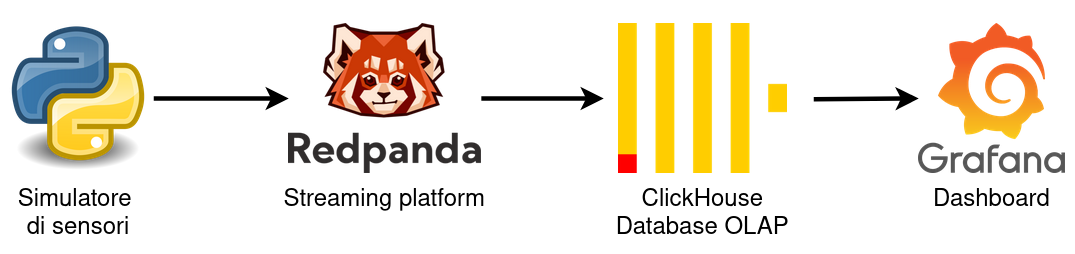
\includegraphics[width=0.8\textwidth]{analisi_dei_requisiti/stack}
	\captionof{figure}{Architettura del prodotto}
\end{center}

\subsection{Funzionalità del prodotto}
Una volta che il sistema sarà in funzione, esso sarà in grado di:
\begin{itemize}
	\item \textbf{Raccogliere} e \textbf{memorizzare} i dati provenienti dai sensori;
	\item \textbf{Visualizzare} i dati raccolti in tempo reale attraverso una \href{https://7last.github.io/docs/rtb/documentazione-interna/glossario\#dashboard}{\textbf{dashboard}\textsubscript{G}}, offrendo una panoramica delle condizioni della città.
	      Tra le informazioni visualizzate ci saranno una mappa con la posizione dei sensori e alcuni grafici che mostrano gli andamenti delle misurazioni;
	\item \textbf{Calcolare} un \textbf{indice di salute} della città, basato sulle ultime rilevazioni dei sensori. Questo indice sarà rappresentato da un punteggio da 0 a 100, dove un punteggio più alto corrisponderà a condizioni di vita migliori;
	\item \textbf{Notificare} automaticamente le autorità locali in caso di superamento di soglie critiche da parte dei sensori.
\end{itemize}

\subsection{Caratteristiche degli utenti}
Si prevede che gli utenti principali saranno i dipendenti delle autorità locali \href{https://7last.github.io/docs/rtb/documentazione-interna/glossario\#responsabile}{responsabili\textsubscript{G}}
del monitoraggio dello stato di salute, sicurezza ed efficienza della città.
Gli utenti interagiscono solamente con il sistema attraverso la \href{https://7last.github.io/docs/rtb/documentazione-interna/glossario\#dashboard}{dashboard\textsubscript{G}}.

\subsubsection{Conoscenze e competenze}
Si suppone che tali utenti siano in grado di comprendere i dati visualizzati dalla \href{https://7last.github.io/docs/rtb/documentazione-interna/glossario\#dashboard}{dashboard\textsubscript{G}} e filtrare le informazioni
per ottenere una visione d'insieme della situazione.

\subsubsection{Dispositivi}
Per accedere alla piattaforma gli utenti potranno indifferentemente utilizzare un dispositivo mobile, un computer o un tablet.






